%% Copyright 1998 Pepe Kubon
%%
%% `two.tex' --- 2nd chapter for thes-full.tex, thes-short-tex from
%%               the `csthesis' bundle
%%
%% You are allowed to distribute this file together with all files
%% mentioned in READ.ME.
%%
%% You are not allowed to modify its contents.
%%

%%%%%%%%%%%%%%%%%%%%%%%%%%%%%%%%%%%%%%%%%%%%%%%%%
%
%     Chapter 5   
%
%%%%%%%%%%%%%%%%%%%%%%%%%%%%%%%%%%%%%%%%%%%%%%%%

\chapter{Spatial Skyline Subspace}
\label{ch:spatial_skyline_subspace}

In this chapter, we will introduce the algorithms to compute the spatial skyline subspace queries. In the computation of spatial skyline subspace skyline queries, we use the same set enumeration framework as shown in Chapter~\ref{ch:graph}. However, in this chapter we introduce a different method to prune the unnecessary \emph{dominating candidates} based on some geometric property of skyline subspace.

\section{Label Collecting in Radius $D$}
We assume that the data points are indexed in R-tree. In R-tree we can get all points in a certain rectangle efficiently. By indexing the data points in R-tree, if we want access the neighbouring points of certain query point $q$, we can query the square with center $q$ in R-tree without accessing the whole set of data points. We compute query point $q$'s label distance vector $LV_q$ by checking the labels of the points in rectangle with upper-left corner point $(p.x - D, p.y - D)$ and lower-right corner point $(p.x + D, p.y + D)$. Then we collect the labels within distance $D$ as the label distance vector $LV_q$.

\section{Dominating Candidates in Spatial Subspace Skyline}

In this section, we will show an algorithm to compute the $\mathit{CAND}$ of all $1$-dimensional subspaces. We enumerate every point $v$ in the data set and build the label distance vector $LV_v$ of the point $v$ by querying square centering in point $v$.

\begin{algorithm}[H]
  \caption{Dominating Candidates}
  \label{algo:spatial_cand}
  \begin{algorithmic}[1]
  \show\LOOP
    \REQUIRE R-tree $R$ that indexes the spatial points and label distance vector $LV_q$ of query point $q$;
    \ENSURE Dominating Candidates Set $\mathit{CAND}$ of all $1$-dimensional subspaces, $\mathit{SDS}$ and $\mathit{EQS}$ of all points;
    \FORALL {$\left(l, dist\right)$ in $LV_q$}
        \FORALL {point $p$ contains label $l$}
            \STATE $rec = R.query(p.x-dist, p.y-dist, p.x+dist, p.y+dist)$
            \FORALL {point $u$ in $rec$}
                \STATE $d$ = $distance(v, p)$
                \IF {$d < dist$}
                    \STATE add$(u, dom)$ to $\mathit{CAND}_l$
                    \STATE add$l$ to $\mathit{SDS}_u$
                \ENDIF
                \IF {$d == dist$}
                    \STATE add$(u, eq)$ to $\mathit{CAND}_l$
                    \STATE add$l$ to $\mathit{EQS}_u$
                \ENDIF
            \ENDFOR
            
        \ENDFOR
    \ENDFOR
  \end{algorithmic}
\end{algorithm}

Consider the Figure~\ref{fig:spatial_map} and \ref{tab:spot_category} as a running example, and let the radius $D = 2$, we compute the label distance vectors of each points by applying Algorithm~\ref{algo:spatial_cand}.

\begin{table}[h]
    \centering
    \begin{tabular}{llll}
    \hline
    Distances & A & B & C \\ \hline
    $u$       & 0 & $\infty$ & $\infty$ \\ \hline
    $v$       & $\sqrt{2}$ & $\infty$ & $\infty$ \\ \hline
    $w$       & $\infty$ & 0 & 0 \\ \hline
    $x$       & $\infty$ & $\infty$ & $\infty$ \\ \hline
    $y$       & $\infty$ & 0 & 1 \\ \hline
    $z$       & $\sqrt{2}$ & 1 & 2 \\ \hline
    \end{tabular}
    \caption{\label{font-table} label distance vector of each points}
    \label{tab:lv_spatial}
\end{table}

\section{Same Region Pruning}
After getting the list of dominating candidate sets and the $\mathit{SDS}$ and $\mathit{EQS}$ of all points, we can prune some unnecessary candidate points of the dominating candidate sets. By Property~\ref{ppt:prune_cand}, we can see that if two points $u$ and $v$ have the same $\mathit{SDS}_u$ and $\mathit{SDS}_v$ and they have the same $\mathit{EQS}_u$ and $\mathit{EQS}_v$, then one of the point $u$ and $v$ can be pruned by the other.

\begin{figure}[h]
    \centering
      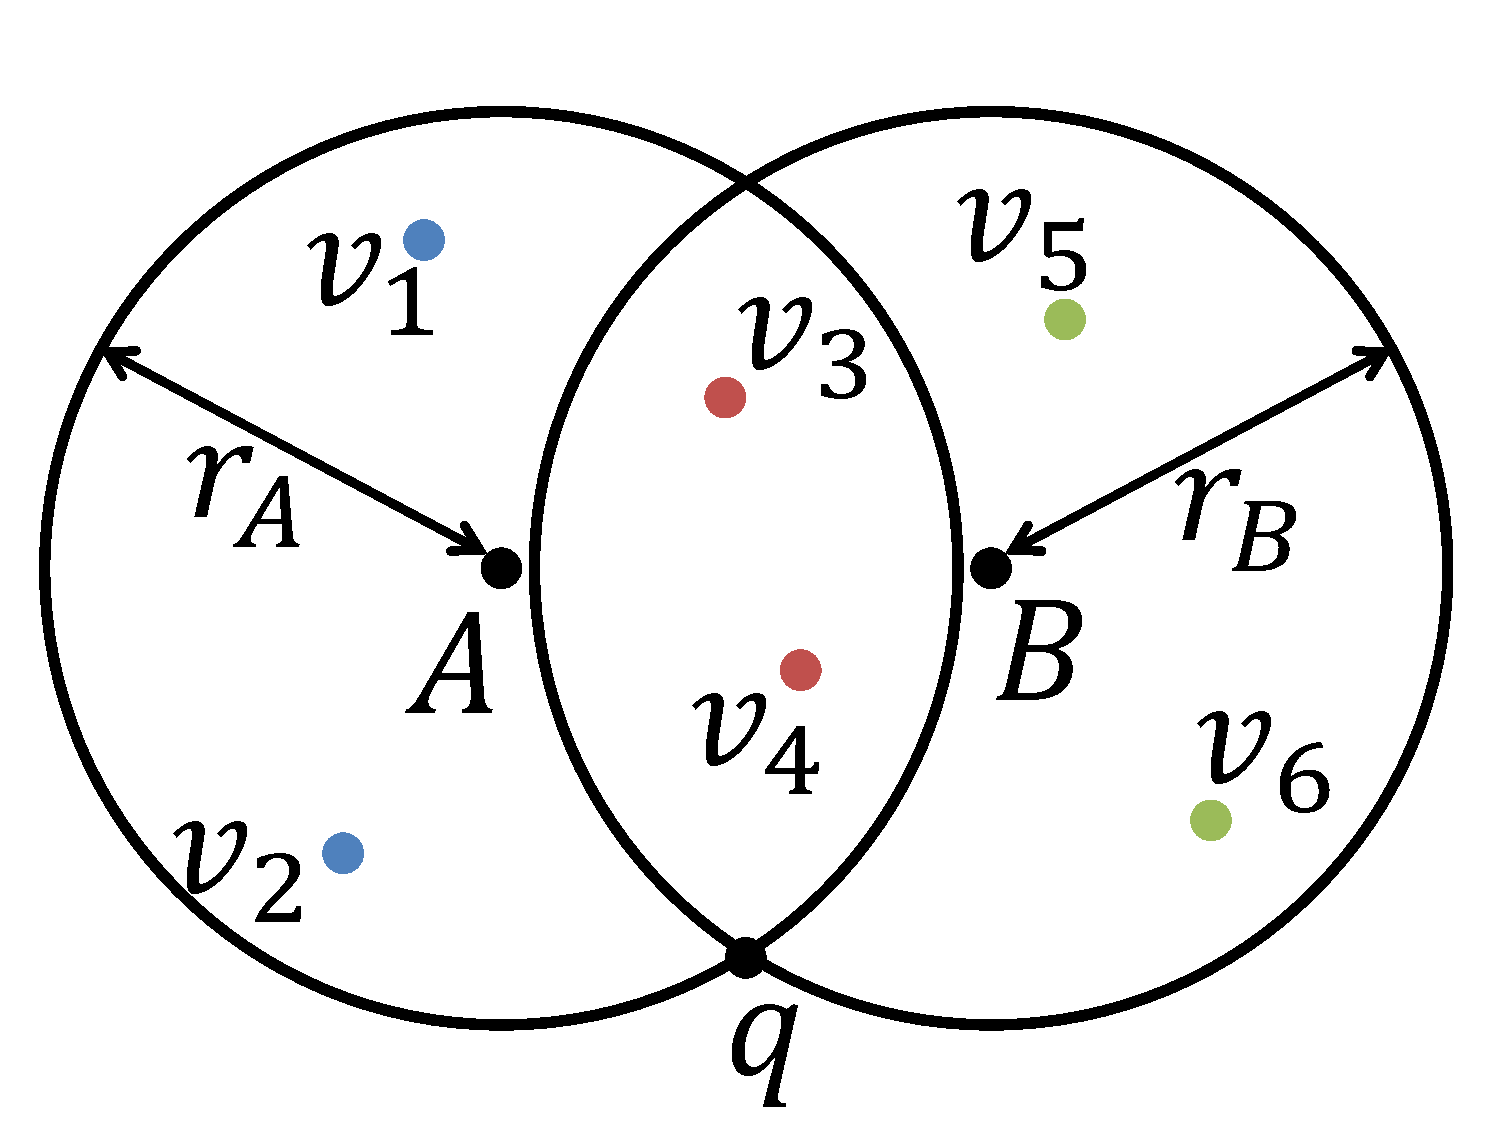
\includegraphics[width=0.4\textwidth]{figs/Circle_Spatial_Example}
    \caption{We can pick one candidate for each region (with same color) and eliminate the others.}
    \label{fig:circle_example}
\end{figure}

We will show an example of how the spatial points can be pruned from the dominating candidate set. In Figure~\ref{fig:circle_example}, point $q$ represents the query point, point $A$ represents a point with label $A$ and point $B$ represents a point with label $B$. $r_{A}$ is the distance between query point $q$ and label $A$ and $r_{B}$ is the distance between query point $q$ and label $B$. The blue points ($v_1$ and $v_2$) dominate the query point $q$ in the $1$-dimensional subspace $A$. The green points ($v_5$ and $v_6$) dominate the query point $q$ in subspace $B$. The red points ($v_3$ and $v_4$) dominate the query point $q$ in subspace $(A, B)$. In this example, the points with the same colors, ($v_1$, $v_2$), ($v_3$, $v_4$), ($v_5$, $v_6$) have the same \emph{strictly dominating subspace} $\mathit{SDS}$ and the same \emph{equivalence subspace} $\mathit{EQS}$. Therefore, we can keep one of them of each color as a representative and prune the others from the \emph{dominating candidate set}.

\begin{property}
\label{ppt:circle_space}
$n$ circle can only divide the $2$-dimensional space into at most $n(n-1)+2$ different regions.
\end{property}

\begin{proof}
Proof by induction.\\
Basic: one circle divide the $2$-dimensional space into $2$ different regions.\\
Inductive step: Assume that the statement stand for $k$, i.e., $k$ circles can only divide the space into at most $k(k-1)+2$ different regions. The $(k+1)$th circle can only intersect with at most $k$ circle with $2k$ intersection points. Then the $(k+1)$th can only be divide into $2k$ segments and each segment divide the region it locates into two. Therefore, $k+1$ circles can only divide the space into at most $k(k-1)+2+2k = k(k+1)+2k$ different regions.\\
Since both the basis and the inductive step have been performed, by mathematical induction, the statement holds for all natural $n$.
\end{proof}

By Property~\ref{ppt:circle_space}, we know that the total number of regions will not be greater than the square of total number of vertices containing label. In practice, the total number of dominating candidates is much less than this number.

\begin{algorithm}[H]
  \caption{Same Region Pruning}
  \label{algo:spatial_prune}
  \begin{algorithmic}[1]
  \show\LOOP
    \REQUIRE Dominating Candidates $CAND$, query vertex $q$, graph $G=(V, E)$;
    \ENSURE Pruned Dominating Candidates $CAND$;
    \FORALL {$(l, dist)$ in $LV_q$}
        \FORALL {$u$ in $CAND_l$}
            \IF {$u$ is in the same region as other points}
                \STATE delete $u$ from $CAND_l$
            \ENDIF
        \ENDFOR
    \ENDFOR
  \end{algorithmic}
\end{algorithm}

After applying the Algorithm~\ref{algo:spatial_prune} to prune the unnecessary element in the \emph{dominating candidate set} in all $1$-dimensional subspace, we will use the same set-enumeration method of skyline subspace computation from Chapter~\ref{ch:graph} to compute the \emph{dominating candidates set} of all subspaces in order to get the spatial skyline subspace.










